\section{Déploiement continu et maintenance}

\subsection{Déploiement}

Nous avons déjà parlé de notre méthode de déploiement dans le lot 1 ainsi que dans \ref{HTTPS}. Nous avons bien mis en place et suivi notre méthode de déploiement du serveur et du client tout au long de notre réalisation de projet.
Pour rappel, l'api est accessible à l'adresse \textbf{\href{https://vroommates-agerard57.herokuapp.com}{https://vroommates-agerard57.herokuapp.com}} et le client se situe sur  \textbf{\href{https://www.vroommates.agerard.dev}{https://www.vroommates.agerard.dev}}. 

\subsection{Cloisonner les environnements}

\begin{figure}[th]
\centering
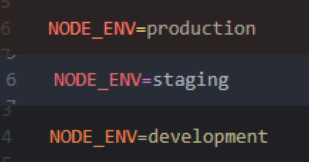
\includegraphics{medias/envExample.png}
\decoRule
\caption{Exemple d'un fichier .env sous 3 environnements différents (dev / staging / production)}
\end{figure}

Nous avons cloisonné les différents environnements pour chaque partie de la plateforme. Au build du code, ce dernier détecte l'environnement sous forme de variable stockée dans les deux fichiers \textbf{.env} du projet (un dans /server, un dans /client).\\
Il existe au total 3 environnements différents:

\begin{itemize}
    \item Nous avons donc l'environnement de "\textbf{development}", qui correspond à la version locale du code. Il s'agit de la version que les développeurs utilisent, afin d'avoir accès aux logs et aux dépendances de développement. 
    \item Ensuite, l'environnement intermédiaire de "\textbf{staging}", correspondant à la branche develop sur Github. C'est ici que l'on teste la compatibilité de nos nouvelles features avant de les publier. Avec chaque pull request de staging vers master, on génère une version test "en ligne", afin de tester dans des conditions se rapprochant plus de l'environnement d'un utilisateur. Cette méthode s'est avéré très efficace pour détecter des bugs ou des erreurs seulement remarquables dans ces conditions. 
    \item Enfin, une fois que nous sommes sûrs qu'il n'y ait ni bugs ni régressions, on déploie notre site, avec l'environnement de "\textbf{production}", correspondant à la branche master.
\end{itemize}

